Now that we've understood classical and quantum mechanics as probability theories and displayed their differences, we will now concern ourselves with the development of algebraic methods that will allow us to describe both classical and quantum mechanics in the same framework and to discuss equilibrium further.
 
\section{C*-algebras}

We will start by getting acquainted with the notion of a C*-algebra. This is the mathematical structure we will endow our physical observables with. Even though the general need for this structure can be inspired by the abstract analysis of experimental apparatuses\cite{Strocchi2008a} we will instead give the abstract definition and then justify it through examples. 

\begin{definition}
An algebra $\mathcal{A}$ is a set equipped with three operations:
\begin{align}
 \mathcal{A} \times \mathcal{A} & \rightarrow  \mathcal{A} \\
 (x,y) & \mapsto  x+y \quad\text{addition;} \nonumber \\
 \mathbb{C} \times \mathcal{A} & \rightarrow \mathcal{A} \\
 (\lambda,x) & \mapsto \lambda x \quad\text{scalar multiplication;} \nonumber \\
 \mathcal{A} \times \mathcal{A} & \rightarrow \mathcal{A} \\
 (x, y) & \mapsto xy \quad\text{multiplication;} \nonumber
\end{align}
such that with addition and scalar multiplication it forms a complex vector space, with addition and multiplication it forms a ring, and there is a compatibility condition between scalar multiplication and multiplication which is that for all $x,y\in\mathcal{A}$ and $\lambda\in\mathbb{C}$ we have $(\lambda x)y=x(\lambda y) = \lambda (xy)$. If the ring is commutative the algebra is said to be commutative and if the ring is unital the algebra is said to be unital. A norm on an algebra $\mathcal{A}$ is a norm on the vector space structure $\|\cdot\|:\mathcal{A} \rightarrow \mathbb{R}^{+}_0 $ such that for all $x,y\in\mathcal{A}$ we have $\|xy\|\leq\|x\|\|y\|$. An algebra endowed with a norm is called a normed algebra. If the normed vector space structure of an algebra is Banach, the algebra is called Banach. An involution on an algebra $\mathcal{A}$ is a map $^*:\mathcal{A}  \rightarrow \mathcal{A} \quad x \mapsto x^*$ such that for all $x,y\in\mathcal{A}$ and $\lambda\in\mathbb{C}$:
\begin{align}
(\lambda x + y)^*&=\bar{\lambda}x^* + y^*; \\
(xy)^*&=y^*x^*;\\
(x^*)^*&=x.
\end{align}
An algebra equipped with an involution is said to be a *-algebra. A $C*$-algebra is a Banach *-algebra where for all $x\in\mathcal{A}$ 
\begin{equation}
\|x^*x\|=\|x\|^2.
\end{equation}
\end{definition}

\begin{example}
The set of continuous functions vanishing at infinity on a locally compact Hausdorff space $X$, that is the set $C_0(X)$ of continuous $f:X\rightarrow \mathbb{C}$ such that for every $\epsilon\in\mathbb{R}^+$ there exists a compact set $K$ such that $f(K^c)\subseteq B(0,\epsilon) \subseteq \mathbb{C}$ forms a $C^*$-algebra with the supremum norm
\begin{equation}
\|f\| = \sup\{|f(x)||x\in X\}.
\end{equation}
This algebra differs from the structure described in \ref{sec:classical_probability} in that the functions are admittedly complex and their behavior at infinity is restricted. Nevertheless $C_0(X)$ is unital if and only if $X$ is compact. In that case $C_0(X)=C(X)$ and the observables coincide with the self-adjoint elements of the $C^*$-algebra. One can associate both the need for restricting behavior at infinity or making the space compact by noting that any real feasible experiment performed on a system should be localized. This has to do with the experimental motivation of $C^*$-algebras given in \cite{Strocchi2008a}.
We now note that every commutative $C^*$-algebra can be realized as the space of continuous functions on a compact Hausdorff space. 
\end{example}

\begin{example}
The set of bounded operators in a Hilbert space $\mathcal{H}$ forms a $C^*$-algebra with the operator norm
\begin{equation}
\|A\|=\sup\left\{\left.\frac{\|Ax\|}{\|x\|}\right|x\in\mathcal{H}\setminus \{0\} \right\}.
\end{equation}
Once again, this algebra differs from the structure given in section \ref{sec:QM} because we only consider bounded operators. Once again at a fundamental level this doesn't matter since we know through the spectral theorem or the logical structure presented in section \ref{sec:Q_logic} that we can describe all observables (bounded or unbounded) through their spectral decomposition into projections. In particular, we should be able to take the $C^*$-algebra generated by the projections associated to the observable we want to analyze. For example, instead of considering the position operator $q$ on $L^2(\mathcal{H})$ given by $q\psi(x)=x\psi(x)$ for all $\psi\in\mathcal{H}$, we can consider the $C^*$-algebra generated by the characteristic functions of Borel sets $E\subseteq\mathbb{R}$ whose action on the Hilbert space is $\chi_E\psi(x) = \chi_E(x)\psi(x)$. Moreover, this problem as in the classical case, this problem is related to the fact that no experimental apparatus has an infinite display of outcomes. One indeed cannot measure infinitely large positions or momenta.

Another solution for the case of Schrödinger's mechanics is to consider the Weyl operators $U(a)$ and $U(b)$ for $a,b\in\mathbb{R}$ given by
\begin{align}
U(a)\psi(x) &= \psi(x-\hbar a) \\
V(b)\psi(x) &= e^{-ibx}\psi(x). 
\end{align}
By Stone's theorem if $q$ is the position operator and $p$ is the momentum operator satisfying the canonical commutation relations $[x,p]=i\hbar$ we have $U(a)=e^{-iap}$ and $V(b)=e^{-ibq}$\cite{Strocchi2008a}. 
\end{example}

As mentioned before the above definition gives structure to the observables of a system. To get a complete kinematical description we need to also give structure to the notion of state. We can inspire the definition of a state by the fact that both in classical and quantum descriptions the statistically appropriate notion of state seemed to act on the observable either through equation \ref{eq:classical_states} or \ref{eq:quantum_states}.

\begin{definition}
A state on a $C*$-algebra $\mathcal{A}$ is a positive normalized linear functional $\omega:\mathcal{A}\rightarrow \mathbb{C}$, i.e. it is a linear map such that $\|\omega\| = 1$ (normalized) and for all $x\in\mathcal{A}$ we have $\omega(x^*x)\geq 0$ (positive).
\end{definition}  

Note that for a unital $C^*$-algebra a positive linear functional $\omega$ is normalized if and only if $\omega(1)=1$.

\begin{example}
By Riesz's representation theorem \cite{Hewitt1975} we have that for every state $\omega$ on $C(X)$ for $X$ compact Hausdorff there exists a probability measure $P$ on $X$ such that
\begin{equation}
\omega (f)=\int fdP
\end{equation}    
for every $f$ in $C(X)$. Indeed $P$ is the measure induced by the Daniel extension of $\omega$. Moreover, it turns out that every commutative $C^*$-algebra is isomorphic to an algebra $C_0(X)$ for $X$ locally compact Hausdorff\cite{Bratteli1997}. In particular, this final remark justifies that classical systems can be treated in the context of $C^*$-algebras. 
\end{example}

\begin{example}
As in the classical case, it so happens that every $C^*-algebra$ can be realized as a closed self-adjoint subalgebra of the algebra of bounded operators of a Hilbert space\cite{Bratteli1997}. This justifies the connection between $C^*$-algebras and the usual presentation of quantum mechanics given in \ref{sec:QM}.
\end{example}

\section{GNS Construction}

Although we won't prove the structure theorems mentioned above for the characterization of $C^*$-algebras we will indeed be interested in the representation of a $C^*$-algebra on a Hilbert space induced by a state. 

\begin{definition}
A representation of a a $C^*$-algebra $\mathcal{A}$ is a tuple $(\mathcal{H},\pi)$ where $\mathcal{H}$ is a Hilbert space and $\pi:\mathcal{A}\rightarrow L(\mathcal{H})$ is a *-homomorphism (i.e. an adjoint preserving homomorphism). If $\mathcal{H}$ has non trivial invariant subspaces under the action of $\pi(\mathcal{A})$ then the representation is said to be reducible.
\end{definition}

\begin{theorem}
If $\mathcal{A}$ is a unital $C^*$-algebra and $\omega$ is a state on it, then there exists a representation $(\mathcal{H}_\omega,\pi_\omega)$ with a unit vector $\Omega_\omega$ such that $\overline{\pi_\omega(\mathcal{A})\Omega_\omega}=\mathcal{H}_\omega$ (i.e., $\Omega_\omega$ is cyclic) and for all $x\in\mathcal{A}$ we have that $\omega(x)=\langle\Omega_\omega,\pi_\omega(x)\Omega_\omega\rangle=tr(\pi_\omega(x)\rho_{\Omega_\omega})$.  
\end{theorem}

\begin{proof}
Notice that in particular $\mathcal{A}$ is a vector space. Consider the function
\begin{align}
\mathcal{A}\times\mathcal{A}&\rightarrow\mathbb{C} \\
(x,y)&\mapsto\omega(x^*y). \nonumber
\end{align}
One can show that this function is an inner product except for the fact that there may be elements $x\in\mathcal{H}\setminus\{0\}$ such that $\omega(x^*x)=0$. We may define $\mathcal{N}_\omega := \{x\in\mathcal{A}|\omega(x^*x)=0\}$. Notice that if $x\in\mathcal{N}_\omega$ and $y\in\mathcal{A}$ then 
\begin{align}
|\omega((yx)^*(yx))|^2&=|\omega(x^*y^*yx)|^2=|\omega((y^*yx)^*x)|^2 \\
&\leq\omega((y^*yx)^*(y^*yx))\omega(x^*x)=0, \nonumber
\end{align}
that is, $\mathcal{N}_\omega$ is a left ideal of $\mathcal{A}$. Notice that now the inner product
\begin{align}
\mathcal{A}/\mathcal{N}_\omega\times\mathcal{A}/\mathcal{N}_\omega&\rightarrow\mathbb{C} \\
([x],[y])&\mapsto\langle[x],[y]\rangle:=\omega(x^*y) \nonumber
\end{align}
is well defined and therefore take $\mathcal{H}_\omega=\overline{\mathcal{A}/\mathcal{N}_\omega}$. We define 
\begin{align}
\pi_\omega:\mathcal{A}&\rightarrow L(\mathcal{H}_\omega) \\
x&\mapsto \pi_\omega(x) \nonumber
\end{align}
by extension of $\pi_\omega(x)[y]:=[xy]$ on $\mathcal{A}/\mathcal{N}_\omega$. We define at last $\Omega_\omega:=[1]$. If $x\in\mathcal{A}$ we have
\begin{equation}\label{eqn:state_representation}
\langle \Omega_\omega, \pi_\omega(x)\Omega_\omega\rangle = \langle \Omega_\omega, [x]\rangle = \omega(x). 
\end{equation}
Moreover $\pi_\omega(\mathcal{A})\Omega_\omega = \mathcal{A}/\mathcal{N}_\omega$ and it is therefore verified that the vector $\Omega_\omega$ is cyclic.  
\end{proof}

\begin{example}\label{example:M2}
Let's follow the GNS construction with the example of the $C^*$-algebra of $2\times 2$ matrices with complex entries $M_2(\mathbb{C})$. This is of physical importance for 2 state systems. For example our recurring system in example \ref{ex:Bell} has this algebra of observables (the canonical matrix representations of the operators $P(0)$, $P(\pi/4)$, $P(\pi/2)$ and $P(3\pi/4)$ generate this algebra). Let the canonical basis of $\mathbb{C}^2$ be $\{e_1, e_2\}$ and the elementary matrices $E_{ij} = ((\delta_{in}\delta_{jm})_{nm})$. Let's choose the state
\begin{equation}
\omega_\lambda(\alpha) = \lambda \alpha_{11} + (1-\lambda)\alpha_{22}
\end{equation} 
for some $\lambda\in [0,1]$. The parameter $\lambda$ can be given interpretation by noting that $\omega_\lambda(P(0))=\lambda$, that is, $\lambda$ is the expectation value of the photon described to have polarization along the horizontal axis. We have that
\begin{align}
\omega_\lambda (\alpha^*\alpha) & = \omega_\lambda\left(\left(\sum_{i=1}^2 (\alpha^*)_{ik}\alpha_{kj}\right)_{ij}\right) = \omega_\lambda\left(\left(\sum_{i=1}^2 \overline{\alpha}_{ki}\alpha_{kj}\right)_{ij}\right) \\
& = \lambda(|\alpha_{11}|^2+|\alpha_{21}|^2) + (1-\lambda)(|\alpha_{12}|^2+|\alpha_{22}|^2). \nonumber
\end{align}
Therefore the ideal $\mathcal{N}_\lambda := \mathcal{N}_{\omega_\lambda}$ will depend on the choice of $\lambda$.
\begin{itemize}
\item If $\lambda = 0$, 
\begin{equation}
\mathcal{N}_0 = \{\alpha\in M_2(\mathbb{C})|\alpha_{12}=\alpha_{22}=0\}.
\end{equation}
Therefore it is clear that if $\mathcal{H}_\lambda:=\mathcal{H}_{\omega_\lambda}$ we have
\begin{equation}
\mathcal{H}_0=M_2(\mathbb{C})/\mathcal{N}_0\simeq\left\{\left.\begin{bmatrix}
0 & \alpha_{12} \\
0 & \alpha_{22}
\end{bmatrix}\right|\alpha_{12},\alpha_{22}\in\mathbb{C}\right\}.
\end{equation}
\item If $\lambda = 1 $ we have the symmetric case and we conclude
\begin{equation}
\mathcal{H}_1=M_2(\mathbb{C})/\mathcal{N}_1\simeq\left\{\left.\begin{bmatrix}
\alpha_{11} & 0 \\
\alpha_{21} & 0
\end{bmatrix}\right|\alpha_{11},\alpha_{21}\in\mathbb{C}\right\}.
\end{equation}
\item If $\lambda \in(0,1)$ we have that $\mathcal{N}_\lambda = \{0\}$ and therefore $M_2(\mathbb{C})/\mathcal{N}_\lambda \simeq M_2(\mathbb{C})$. We have in particular that this representation can be decomposed into the two previous representations
\begin{equation}
M_2(\mathbb{C})=\left\{\left.\begin{bmatrix}
0 & \alpha_{12} \\
0 & \alpha_{22}
\end{bmatrix}\right|\alpha_{12},\alpha_{22}\in\mathbb{C}\right\}\oplus\left\{\left.\begin{bmatrix}
\alpha_{11} & 0 \\
\alpha_{21} & 0
\end{bmatrix}\right|\alpha_{11},\alpha_{21}\in\mathbb{C}\right\}.
\end{equation} 
Moreover, if $\alpha \in M_2(\mathbb{C})$ we have
\begin{equation}
(\pi_{\Omega_{\omega_\lambda}}(\alpha)E_{ij})_{nm}=\sum_{k=1}^2\alpha_{nk}\delta_{ik}\delta_{jm}=\alpha_{ni}\delta_{jm}
\end{equation}
and therefore the spaces in the decomposition are invariant under the action of the representation of the algebra. In particular, we check that the projection $\rho_{\Omega_{\omega_\lambda}}$ onto $\Omega_{\omega_\lambda}$ cannot be of the form $\pi_{\Omega_{\omega_\lambda}}(\alpha)$ for some $\alpha\in M_2(\mathbb{C})$ since it doesn't respect that invariance
\begin{equation}
\rho_{\Omega_{\omega_\lambda}}(E_{ij})=\langle \Omega_{\omega_\lambda}, E_{ij}\rangle\Omega_{\omega_\lambda} = \omega_\lambda(E_{ij})I_2=(\lambda\delta_{1i}\delta_{1j}+(1-\lambda)\delta_{2i}\delta_{2j})I_2.
\end{equation} 
\end{itemize}
\end{example}

Given equation \ref{eqn:state_representation} one may feel tempted to associate to the system the orthogonal projection $\rho_{\Omega_{\omega_\lambda}}$ onto $\Omega_{\omega_\lambda}$ as a state. This would yield according to equation \ref{eqn:entropy_pure} a state of zero entropy. We need to find a way around this. Now, examining our previous example where the state was conveniently written as a convex sum of states, we find that the extremal points of this sum (the cases $\lambda\in\{0,1\}$) generate irreducible representations of the algebra while the other cases didn't. Moreover, the actual state $\rho_{\Omega_{\omega_\lambda}}$ was not in the image of the algebra of observables in the reducible representations considered. This inspires us to try to find a state $\rho_{\omega_\lambda}$ which also satisfies $tr(\pi_{\omega_lambda}(\alpha)\rho_{\omega_\lambda})=\omega(\alpha)$ from the irreducible representations in the GNS construction.

Being concerned for the moment with finite dimensional representations, we will in general be able to write
\begin{equation}
\mathcal{H}_\omega = \bigoplus_{\beta\in I}\mathcal{H}_\omega^{(\beta)}
\end{equation}
where $\{\mathcal{H}_\omega^{(\beta)}|\beta\in I\}$ is a set of irreducible representations of $\mathcal{A}$. The decomposition leaves the projection operators $P^{(\beta)}$ onto $\mathcal{H}_\omega^{(\beta)}$ such that
\begin{equation}
id_{\mathcal{H}_\omega}=\sum_{\beta\in I}P^{(\beta)}.
\end{equation}
Therefore, we have if $\{e_1,\cdots,e_n\}$ is a basis for $\mathcal{H}_\omega$
\begin{align}
\omega(\alpha)&=\langle \Omega_\omega, \pi_\omega(\alpha)\Omega_\omega\rangle \\
&=\langle\Omega_\omega,\sum_{\beta\in I}P^{(\beta)}\pi_\omega(\alpha)\Omega_\omega\rangle \\
&=\langle\Omega_\omega,\sum_{\beta\in I}P^{(\beta)}\pi_\omega(\alpha)P^{(\beta)}\Omega_\omega\rangle \\
&=\langle\Omega_\omega,\sum_{m=1}^n\langle e_m,\sum_{\beta\in I}P^{(\beta)}\pi_\omega(\alpha) P^{(\beta)}\Omega_\omega\rangle e_m\rangle \\
&=\sum_{m=1}^n\langle e_m,\sum_{\beta\in I}P^{(\beta)}\pi_\omega(\alpha) P^{(\beta)}\langle\Omega_\omega, e_m\rangle\Omega_\omega\rangle \\
&=\sum_{m=1}^n\langle e_m,\sum_{\beta\in I}P^{(\beta)}\pi_\omega(\alpha) P^{(\beta)}\rho_{\Omega_\omega} e_m\rangle \\
&=tr(\sum_{\beta\in I}P^{(\beta)}\pi_\omega(\alpha) P^{(\beta)}\rho_{\Omega_\omega})\\
&=tr(\pi_\omega(\alpha)\sum_{\beta\in I}P^{(\beta)}\rho_{\Omega_\omega} P^{(\beta)}).
\end{align}
Therefore we define
\begin{equation}
\rho_\omega := \sum_{\beta\in I}P^{(\beta)}\rho_{\Omega_\omega} P^{(\beta)}
\end{equation}
as the induced state.

\begin{example}
Continuing with example \ref{example:M2} we find that since in the cases $\lambda\in\{0,1\}$ since the representation is irreducible we have $\rho_{\omega_\lambda}=\rho_{\Omega_{\omega_\lambda}}$ and therefore the state is pure and has null entropy. In the case $\lambda\in (0,1)$ we have for all $\alpha\in M_2(\mathbb{C})$
\begin{align}
\rho_{\omega_\lambda}\alpha &= \sum_{i=1}^2 P^{(i)}\rho_{\Omega_{\omega_\lambda}}P^{(i)}\alpha \\
& = P^{(1)}\rho_{\Omega_{\omega_\lambda}}\begin{bmatrix}
\alpha_{11} & 0 \\
\alpha_{21} & 0 
\end{bmatrix} + P^{(2)}\rho_{\Omega_{\omega_\lambda}}\begin{bmatrix}
0 & \alpha_{12} \\
0 & \alpha_{22} 
\end{bmatrix} \\
& = P^{(1)}\omega\left(\begin{bmatrix}
\alpha_{11} & 0 \\
\alpha_{21} & 0 
\end{bmatrix} \right)I_2 + P^{(2)}\omega\left(\begin{bmatrix}
0 & \alpha_{12} \\
0 & \alpha_{22} 
\end{bmatrix} \right)I_2 \\
&= P^{(1)}\lambda\alpha_{11}I_2 + P^{(2)}(1-\lambda)\alpha_{22}I_2 =\lambda\alpha_{11} E_{11} + (1-\lambda)\alpha_{22}E_{22} \\
& = \lambda\rho_{E_{11}}\alpha + (1-\lambda)\rho_{E_{22}}\alpha = (\lambda\rho_{E_{11}} + (1-\lambda)\rho_{E_{22}})\alpha
\end{align} 
and therefore $\rho_{\omega_\lambda}=\lambda\rho_{E_{11}} + (1-\lambda)\rho_{E_{22}}$.
We conclude that the entropy is 
\begin{equation}\label{eq:entropy_M2}
S = \lambda\log (\lambda) + (1-\lambda)\log(1-\lambda)
\end{equation}
\begin{figure}
\centering
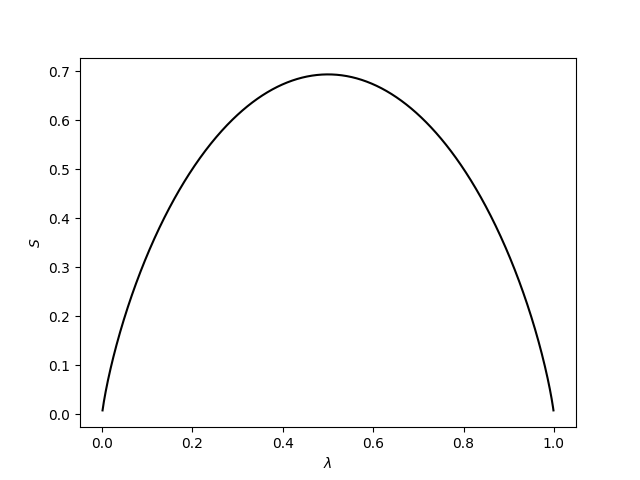
\includegraphics[width=0.8\textwidth]{entropia_M2.png}
\caption{The entropy of equation \ref{eq:entropy_M2} as a function of the probability that the photon has horizontal polarization.}
\end{figure}
\end{example}